

%%%%%%%%%%%%%%%%%%%%%%%%%
 \section{Study Case}

   \begin{frame}
    \frametitle{Outline}
    \begin{columns}[T]
        \begin{column}{.45\textwidth}
            \tableofcontents[sections=1-3,currentsection]
        \end{column}
        \begin{column}{.45\textwidth}
            \tableofcontents[sections=4-5,currentsection]
        \end{column}
    \end{columns}
    \end{frame}

\subsection{Problem Geometry}
\begin{frame}{\subsecname}
Three-bladed propeller equipped with a left-handed Varioprop 12C 3-blades (diameter = 300 mm) \cite{tesis}  \cite{paper}.
\begin{figure} [H]  
	\centering
	\subfloat[Side-by-side]
	{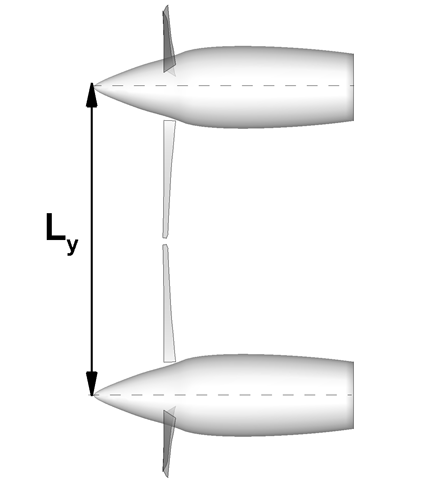
\includegraphics[scale=0.3]{Photos/side-by-side.png}
  }
  \quad
	\subfloat[Tandem]
	{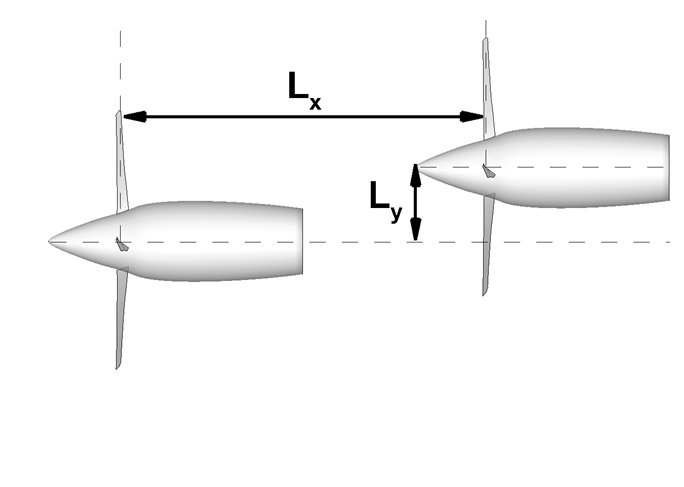
\includegraphics[scale=0.2]{Photos/tandem.png}
  }
\end{figure} 
\vspace{-0.5cm}
 \begin{table}[H]
                %\caption*{\textbf{Title of Table (optional)}}
                \centering 
                \begin{tabular}{|c c c |}
                \hline
                \rowcolor{bluePoli!40 } % bluePoli!40 comment this line to remove the color
                  & $L_x$ [m] & $L_y$ [m]  \T\B \\
                \hline \hline
                Side-by-Side Props & 0 & [0.31 0.40]\T\B  \\
                Tandem Props & 0.1 & [0.25 0.31]\T\B  \\
                \hline
                \end{tabular}
    \end{table}
\end{frame}

\begin{frame}{\subsecname}
    \begin{figure} [H]  
	\centering
	\subfloat [040.000]
	{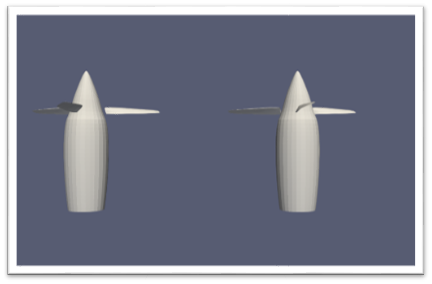
\includegraphics[scale=0.35]{Photos/040.000.png}}
  \quad
	\subfloat [031.010]
	{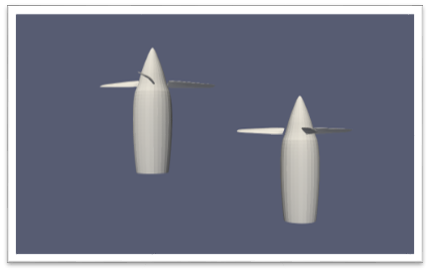
\includegraphics[scale=0.35]{Photos/031.010.png}}
  \quad
	\subfloat [031.000]
	{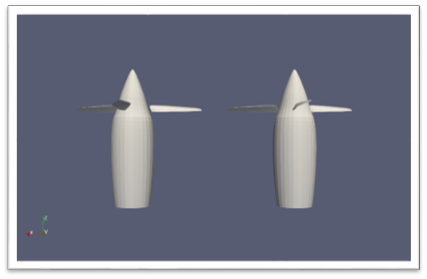
\includegraphics[scale=0.35]{Photos/031.000.png}}
   \quad
	\subfloat [025.010]
	{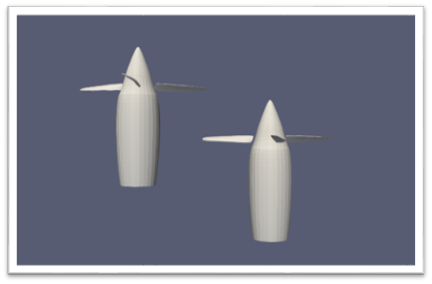
\includegraphics[scale=0.35]{Photos/025.010.png}}
\end{figure} 
\end{frame}

\subsection{Setup}
\begin{frame}{\subsecname}
\begin{itemize}
    \item $V_\inf$ = 28 m/s \& $M_a$ = 0.082
    \item $\omega$ = 738 rad/s
    \item Tip Mach Number \xrightarrow{} $M_t$ = 0.32 
    \item Propellers aligned to the freestream velocity vector
\end{itemize}
\end{frame}


